As we have seen with all of these other topics in angular mechanics, there is a clear connection between the angular and translation formulas. Angular work and power are no different. We think of angular work as being the work necessary to make an object spin for a certain period of time. Then angular power becomes the rate of work that is necessary to make the object spin at the rate that it is spinning it. Before we analyze any examples, let us find the correct formula for angular work. We know that the integral of force over a certain distance is equal to work so we can use our angular versions of force and distance to plug in and find our version of angular work. We find that the integral of torque over changes in the angle of rotation is equal to the angular version of work. Symbolically, that is \begin{equation}W_{angular} = \int \tau d\theta\end{equation}
We know that power is simply the time derivative of work so we can say that same thing for angular work. Lastly, we know that at a constant force, translational power is equal to $Fv$. We can replace both of these terms with their angular counterparts to find the angular versions of these formulas. We find that $P_{angular} = \tau \omega$

Now that we have these formulas down we will do some examples. 
First, let us find the power that must be delivered to a disk(assuming a perfectly flat disk) of mass M and radius R to allow it to rotate at an angular velocity omega w starting from rest in a time t. We know that the torque is equal to the moment of inertia of the disk times the angular acceleration of the disk. We will take the angular acceleration to be constant as the power being delivered to the disk is constant. We can use our equation for the angular velocity of an accelerating object $\omega_f=\omega_i+\alpha t$. Where $\alpha$ is the angular acceleration and $\omega$ is the angular speed. We assume that the initial angular velocity will be 0, so we have that $\frac{\omega_f}{t}$ is the angular acceleration. So $\alpha =\frac{\omega}{t}$. We also know that the moment of inertia for a flat disk is equal to $\frac{MR^2}{2}$. So we have the torque acting on the disk is equal to $\frac{M\omega R^2}{2t}$. We also know that from our formula for angular power, the power being delivered to the disk is equal to the torque times the angular velocity, so we find that \begin{equation}P = \frac{M\omega^2 R^2}{2t}\end{equation} Now, we need to check that this makes sense. First, it makes sense that if we can spend longer delivering power to the disk, we have to deliver less at each instant. Additionally, it would make sense that if we have a disk with a higher moment of inertia, that it is as if it was heavier and therefore would require more power to get it going at a certain speed. Lastly, it is obvious that if we want the disk to spin at a higher speed, assuming everything else is constant, we are going to have to deliver more power to the disk. We can use this formula for power to find out how much work it would take to accelerate the disk to the given angular velocity. We have to take the integral of the power with respect to time. However, before you begin integrating our expression with respect to time, it is essential to understand that our variable $t$ is the total time that it takes to accelerate our disk and not the time that has elapsed since we began accelerating the disk. If t were changing in time, then the power being delivered to the disk would not be constant, and this is not what we want. When we take the integral correctly, we find that the work that must be done to the disk is equal to $\frac{M\omega^2R^2}{2}$. This makes sense as it is just the rotational kinetic energy of the disk when it reaches the angular velocity w. Overall, angular work and power are relatively simple concepts once we understand their translational forms and the problems can mainly get harder if we assume a more complex system, but usually solving these requires more math than physics. For example, how much power does it take to get the water in a cup to move at angular velocity $v$ uniformly around the center of the cup in the horizontal plane? We can assume that the water is in the shape of a funnel, which we can model as a cone. An image is shown in Fig. 6.6.1.
\newline
\newline
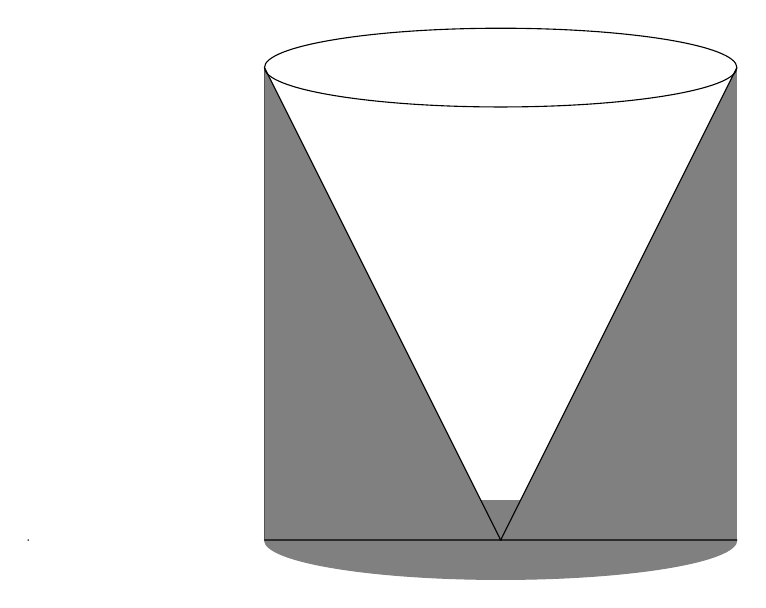
\begin{tikzpicture}
\draw (0,0) circle(0.0001cm);
\filldraw[fill = gray, draw=gray] (6,0) ellipse(3cm and 0.5 cm);
\draw (3,0) -- (3,6);
\draw (9,0) -- (9,6);
\filldraw[fill = gray, draw=black] (3,6) -- (6,0) -- (3,0);
\filldraw[fill = gray, draw=black] (9,6) -- (6,0) -- (9,0);
\draw (6,6) ellipse(3cm and 0.5 cm);
\end{tikzpicture}
\newline
\newline
\begin{center}
(Figure 6.6.1)
\end{center}